%------------------------------------------------------------------------------
\begin{frame}
  \frametitle{Probl\`eme physique}
  %JE VAIS
  Calculer les tensions $U(z,\omega) =(u_1 \cdots u_N)^T$ et les courants
  $I(z,\omega) = (I_1\cdots I_N)$ complexes dans un faisceau de conducteurs
  $w_i$, $i=1\cdots N$. Les cables sont entour\'es d'un blindage $w_0$. La forme
  du faisceau est fix\'ee dans le plan $(x,y)$ et invariante suivant $z$.
  \begin{center}
    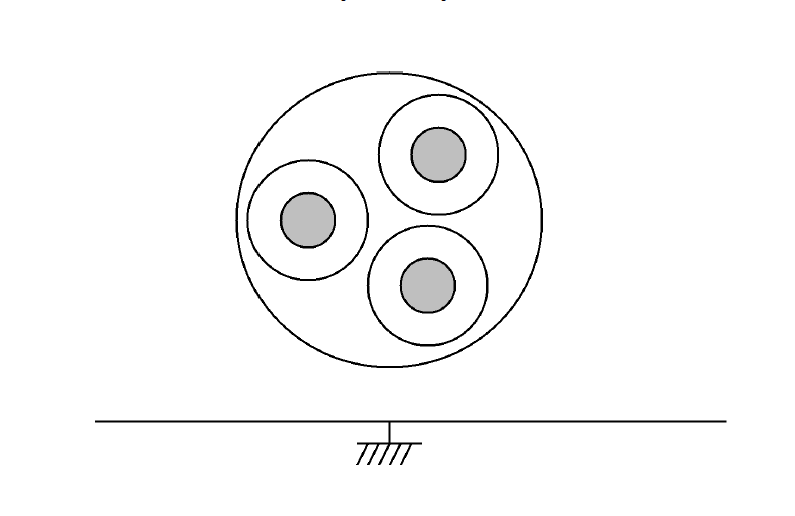
\includegraphics[height=4cm]{figures/f1}\\
    \small  Exemple de section d'un cable.
  \end{center}
\end{frame}
%------------------------------------------------------------------------------


\begin{frame}
\frametitle{Ligne de transmission}
\'Equation des lignes de transmissions ($j^2=-1$)
\begin{eqnarray*}
\frac{\partial U}{\partial z} =ZI, \quad Z=R+j\omega L,\\
\frac{\partial I}{\partial z} =YU, \quad Y=G+j\omega C.
\end{eqnarray*}
Matrices: 
Imp\'edance $Z$, R\'esistance $R$, Inductance $L$, Admittance $Y$, Conductance $G$, Capacit\'e
$C=L^{-1}.$\\[0.4cm]
Propri\'etes des matrices: 
\begin{itemize}
\item Sym\'etrique
\item D\'efinie positive
\end{itemize}

\end{frame} 

\begin{frame}
\frametitle{Probl\`eme}
Flux magn\'etique $\varphi(x,y)$. \\
Champ magn\'etique: d\'edrive d'un potentiel vecteur 
$$B=\nabla \times (0,0,\varphi)^T.$$ et
$$\nabla\times B=(0,0,j_z)^T$$ avec
\begin{itemize}
\item  $j_z(x,y)$ : densit\'e de courant suivant $z$
\item  $I_i= \int _{w_i}j_z(x,y)dxdy$ :  courant
\end{itemize}
On a
\begin{equation}
-\Delta\varphi =
\begin{cases}
j_z \\ 
0 \qquad \text{sur } \Omega =w_0 \setminus \cup_i w_i,
\end{cases}
\end{equation} 
\end{frame}

